\documentclass{standalone}
\usepackage{tikz}
\usepackage{pgfplots}
\pgfplotsset{width=32cm,height=18cm,compat=1.3}
\pgfplotsset{every tick label/.append style={font=\Huge}}
\usepackage{filecontents}

\usetikzlibrary{patterns}

\definecolor{citrine}{rgb}{0.89, 0.82, 0.04}

\begin{document}
	\centering
		\vspace{1.5em}
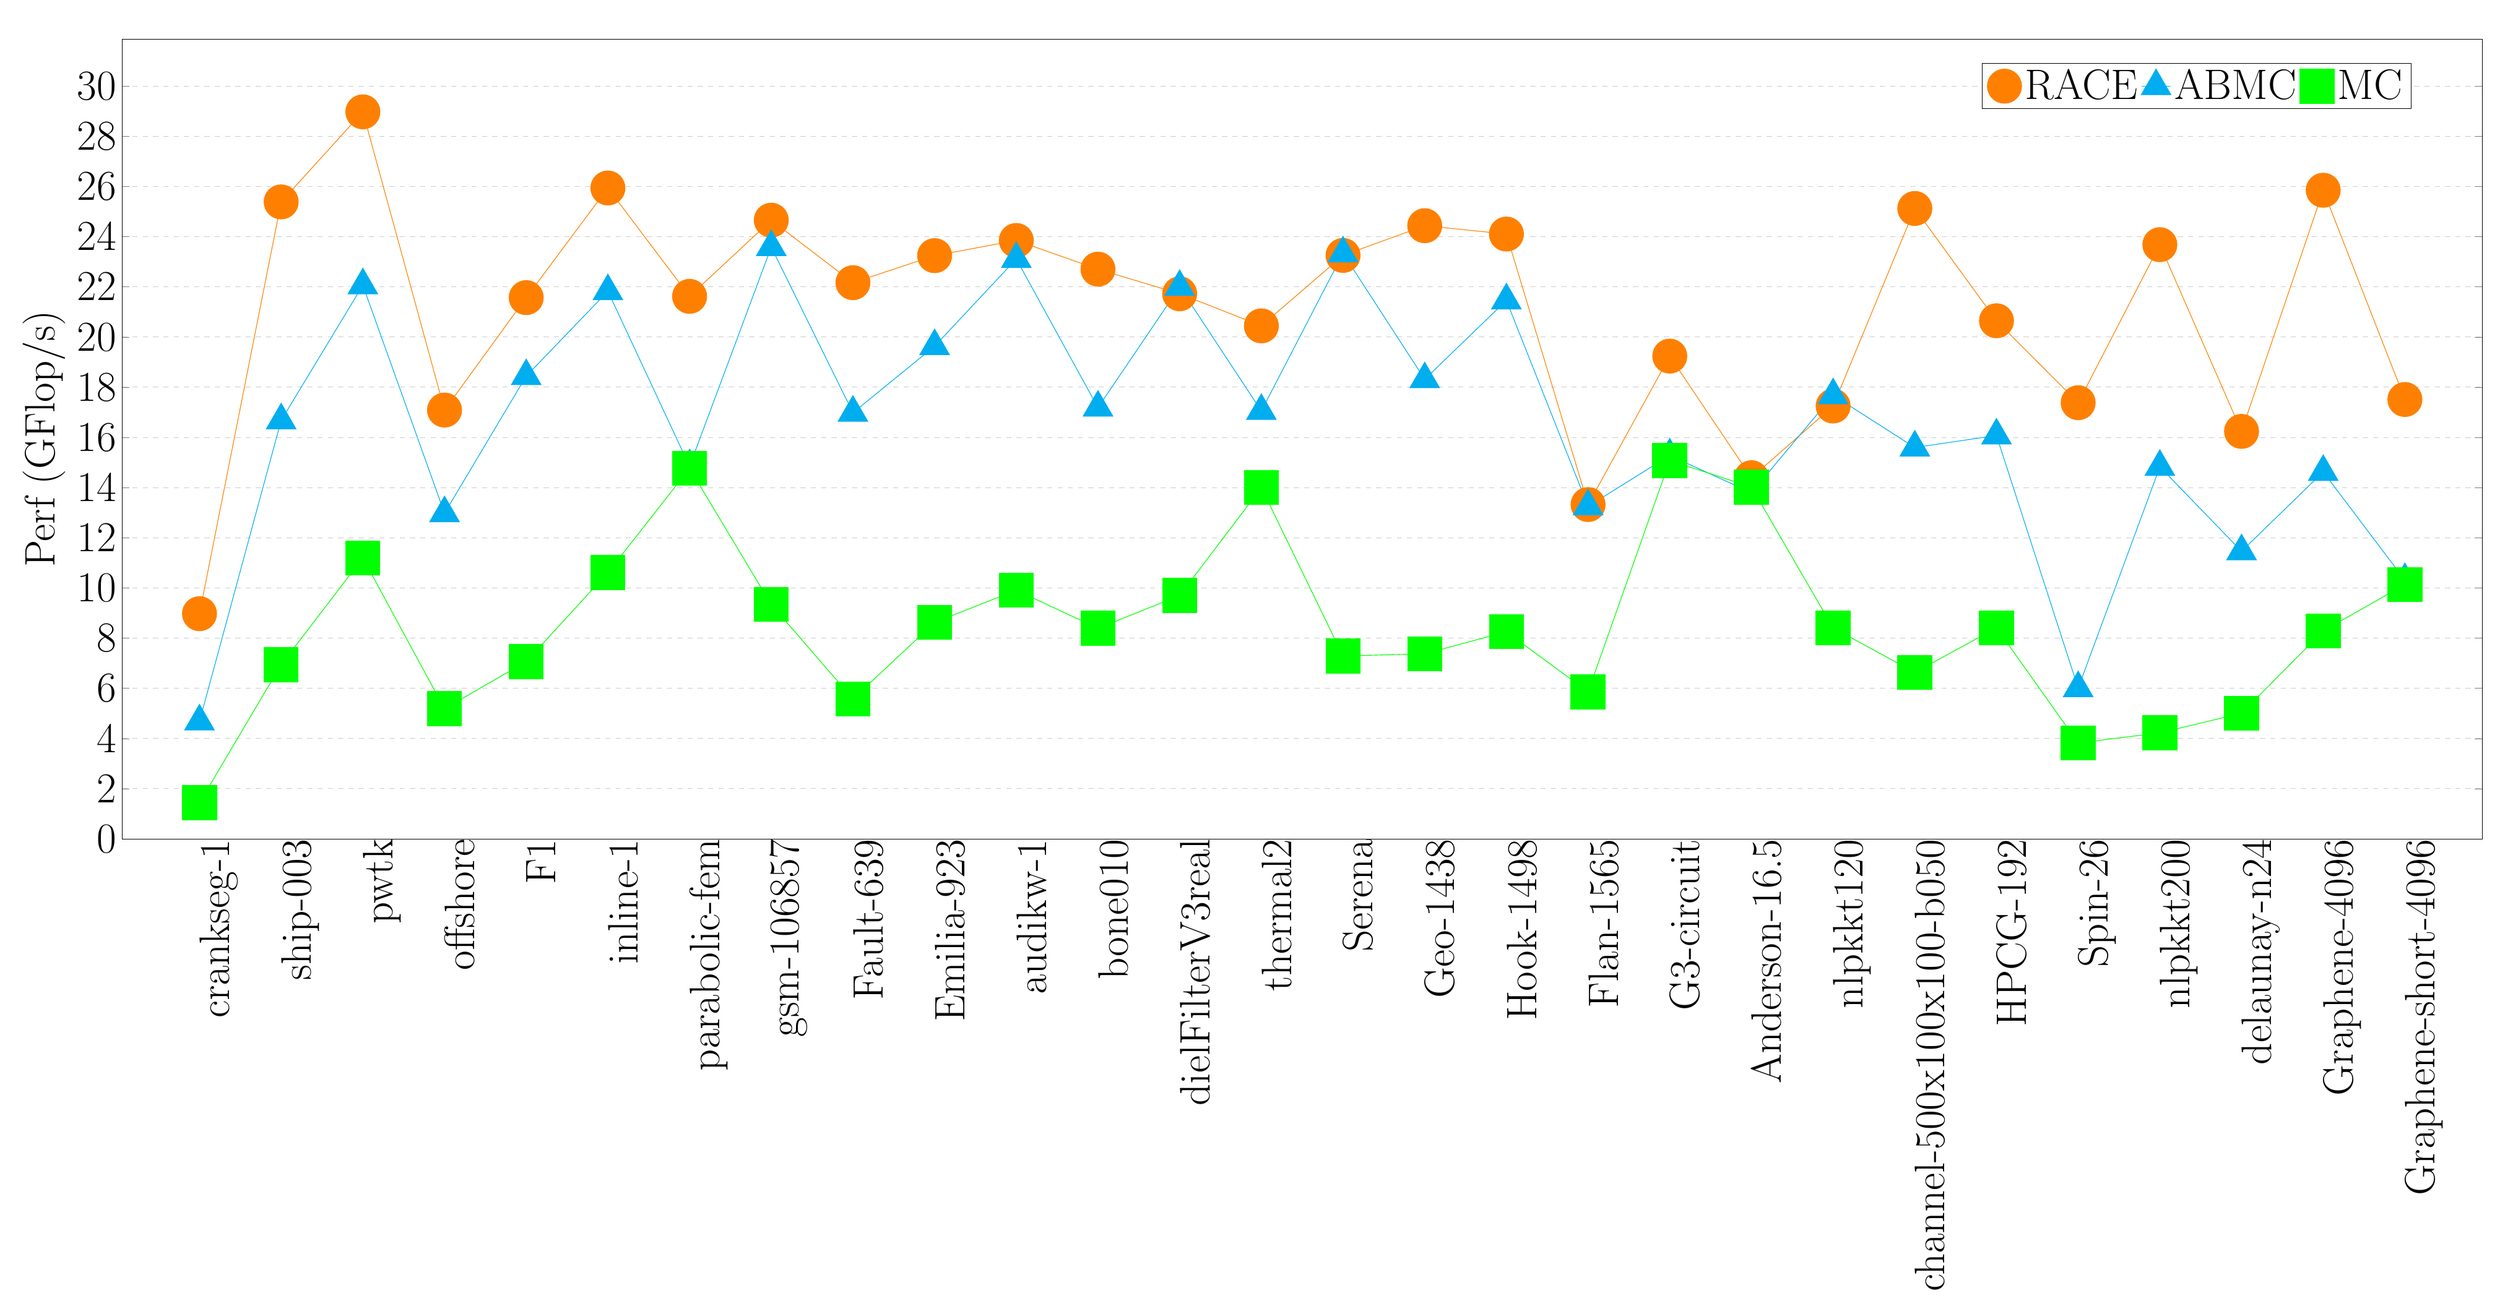
\begin{tikzpicture}
		%	\node at (13.25,15) {\LARGE{}};
			\begin{axis}[
		%	xmin=0.25, xmax=7.25,
			ymin=0, %ymax=3.25,
			xtick={1, 2, 3, 4, 5, 6, 7, 8, 9, 10, 11, 12, 13, 14, 15, 16, 17, 18, 19, 20, 21, 22, 23, 24, 25, 26, 27, 28},
		%	ytick={0,0.5,1,1.5,2,2.5,3},
			xticklabels={crankseg-1, ship-003, pwtk, offshore, F1, inline-1, parabolic-fem, gsm-106857, Fault-639, Emilia-923, audikw-1, bone010, dielFilterV3real, thermal2, Serena, Geo-1438, Hook-1498, Flan-1565, G3-circuit, Anderson-16.5, nlpkkt120, channel-500x100x100-b050, HPCG-192, Spin-26, nlpkkt200, delaunay-n24, Graphene-4096, Graphene-short-4096},
			width  = 50cm,
			height = 18cm,
			major x tick style = transparent,
			%	minor ytick={1, 5, 10, 15, 20, 25, 30 ,35,40},
			grid = minor,	
			%add_bar_commands
			ymajorgrids = true,
			grid style={dashed, gray!40},
			ylabel = {\Huge{Perf (GFlop/s)}},
		%	symbolic x coords={Graphene-2048-2048, Graphene-4096-4096, Spin-24-24-24},
			x tick label style={rotate=90, anchor=north east, inner sep=0mm, font={\Huge}},
			tick label style={font={\Huge}},
			scaled y ticks = false,
			enlarge x limits=0.035,
			legend cell align=left,
			legend style={font=\Huge},
			legend columns=-1,
			legend style={
				%at={(1,1.05)},
				%anchor=south east,
				%column sep=1ex,
				legend pos=north east
			},
			%spl_legend_code
			title= {\Huge\scalebox{1.5}{{}}}
			]

\addplot[ mark=*, mark size=10pt, mark options={orange}, draw=orange , y filter/.code={\pgfmathparse{\pgfmathresult*1000}\pgfmathresult}] plot coordinates{(1,.00897509803921568627) (2,.02538524757281553398) (3,.02897395242718446601) (4,.01708972524271844660) (5,.02157063921568627450) (6,.02593908500000000000) (7,.02162083619047619047) (8,.02465642475247524752) (9,.02216613706896551724) (10,.02324384424778761061) (11,.02384841078431372549) (12,.02270439047619047619) (13,.02172377352941176470) (14,.02044520396039603960) (15,.02325289081632653061) (16,.02443641730769230769) (17,.02410411250000000000) (18,.01332391459459459459) (19,.01923930761904761904) (20,.01439394308943089430) (21,.01725093928571428571) (22,.02512337475728155339) (23,.02064791250000000000) (24,.01738307383177570093) (25,.02368053203883495145) (26,.01624013592233009708) (27,.02584987821782178217) (28,.01751016534653465346)};
\addplot[ mark=triangle*, mark size=10pt, mark options={cyan}, draw=cyan , y filter/.code={\pgfmathparse{\pgfmathresult*1000}\pgfmathresult}] plot coordinates{(1,.00468051985294117647) (2,.01667937064220183486) (3,.02206170256410256410) (4,.01297845490196078431) (5,.01844180185185185185) (6,.02182517431192660550) (7,.01484992320000000000) (8,.02358385728155339805) (9,.01698136095890410958) (10,.01963661742424242424) (11,.02310876132075471698) (12,.01718702285714285714) (13,.02199612142857142857) (14,.01705493809523809523) (15,.02333291200000000000) (16,.01831643636363636363) (17,.02145892773109243697) (18,.01325256349206349206) (19,.01528002843137254901) (20,.01379608125000000000) (21,.01767845983606557377) (22,.01559626967213114754) (23,.01607676585365853658) (24,.00600553771929824561) (25,.01482691532258064516) (26,.01146261206896551724) (27,.01462416666666666666) (28,.01031155350877192982)};
\addplot[ mark=square*, mark size=10pt, mark options={green}, draw=green , y filter/.code={\pgfmathparse{\pgfmathresult*1000}\pgfmathresult}] plot coordinates{(1,.00144019370078740157) (2,.00694506637168141592) (3,.01119501735537190082) (4,.00518759916666666666) (5,.00706505440000000000) (6,.01061268514851485148) (7,.01476551048951048951) (8,.00934010909090909090) (9,.00557825030674846625) (10,.00862392721088435374) (11,.00991139797979797979) (12,.00839198024691358024) (13,.00969757936507936507) (14,.01399817058823529411) (15,.00728826991150442477) (16,.00737592075471698113) (17,.00825562957746478873) (18,.00585814673913043478) (19,.01507801818181818181) (20,.01402132213740458015) (21,.00840721969696969696) (22,.00663392374100719424) (23,.00841156544117647058) (24,.00382433023255813953) (25,.00422507910447761194) (26,.00500671962025316455) (27,.00828739034482758620) (28,.01013535798319327731)};
	%addplot cmd

	\legend{RACE, ABMC, MC}

	\end{axis}			
\end{tikzpicture}

\end{document}

